
\documentclass[]{article}
\voffset=-1.2cm
\oddsidemargin=0.0cm
\textwidth = 470pt
\usepackage[utf8]{inputenc}
\usepackage[english]{babel}
\usepackage{framed}
\usepackage{graphicx}
\usepackage{enumerate}% http://ctan.org/pkg/enumerate
\usepackage{multicol}
\usepackage{amsmath}
\usepackage{amssymb}
%=========================================================================================== %

\begin{document}


\section*{MA4702 - Fundamentals of Mathematics and Limits}
%=============================== %

\noindent \textbf{Notation:}
\begin{framed}
	\begin{multicols}{2}
		\begin{itemize}
			\item $\mathbb{R}$ - All real numbers positive and negative
			\item $\mathbb{R}^+$ - All positive real numbers including $0$
			\item $\mathbb{R}^-$ - All negative real numbers including $0$
			\item $[a,b]$ - All real numbers $x$ such that $a \le x \le b$
			\item $(a,b)$ - All real numbers $x$ such that $a < x < b$
			\item $[a,\infty)$ - All real numbers $x$ such that $a \le x$
			\item $(a,\infty)$ - All real numbers $x$ such that $a < x$
		\end{itemize} 
	\end{multicols}
\end{framed}


\subsection*{Question 1 : Evaluation of Functions}
	
	\begin{itemize}
		\item[(i)] Evaluate the following function for x = -1,0,1 and 2 respectively.
		{
			\Large
			\[ f(x) = \frac{e^x - {e^{-x}}}{2} \]
		}
		\item[(ii)] Evaluate the function for each of the following values : $0.5,\;1,\;1.25,\;2$.
		{
			\Large
			\[f(x) =  \sqrt{1+e^{x}}  \]
		}
	\end{itemize}
	\subsection*{Question 2 : Floor and Ceiling Functions (Part A)}
\begin{framed}	\begin{itemize}
		\item $\lceil x\rceil$ : Ceiling function
		\item $\lfloor x\rfloor$  : Floor Function
		\item $\{x\}$ : Fractional Part of a number
		($\{x\} = x- \lfloor x\rfloor$)
	\end{itemize}
\end{framed}	\bigskip
	Complete the following table.
	\begin{center}
		{ \large 
			\begin{tabular}{|c|c|c|c|} \hline
				Value x & Floor $\lfloor x\rfloor$ & Ceiling  $\lceil x\rceil$ & Fractional $ \{ x \} $\\ \hline
				-1.4  &	-2	&-1&	 \\ \hline
				2.3&	&		& \\ \hline
				7/9&		&		& \\ \hline 
				-16/3&		&		& \\ \hline
				0 & 	&		& 0 \\ \hline
				1 & 	&	1	& \\
				\hline
			\end{tabular} 
		}
	\end{center}
	\bigskip
	\subsection*{Question 3 : Floor and Ceiling Functions (Part B)}
	Provide some values for $x$ and $y$ that \textbf{contradict} the following statement.
	\[ \lfloor x + y \rfloor  = \lfloor x\rfloor + \lfloor y \rfloor\]
	
	\noindent If the values of x and y were integers, would the equation be true for all values of $x$ and $y$?
	
	%------------------------------- % 



	\subsection*{Question 4 : Laws for Logarithms}
	The following laws are very useful for working with logarithms.\bigskip
	\begin{framed}
	\begin{multicols}{2}
	\begin{enumerate}
		\item $\mbox{log}_b(X)$ + $\mbox{log}_b(Y)$ = $\mbox{log}_b(XY)$\bigskip
		\item $\mbox{log}_b(X)$ - $\mbox{log}_b(Y)$ = $\mbox{log}_b(X / Y)$ \bigskip
		\item $\mbox{log}_b(X^Y)$ = $Y \mbox{log}_b(X)$
		
		\item $\mbox{log}_b(X) = 1 $ when $b=X$
	\end{enumerate}
	\end{multicols}
	\end{framed}

\bigskip
\large
\noindent Use the Laws of Logarithms to evaluate the following expressions:

	\begin{multicols}{2}
		\begin{itemize}
		\item[(i)] $\mbox{log}_2(8)$
		\item[(ii)] $\mbox{log}_2(\sqrt{128})$
		\item[(iii)] $\mbox{log}_2(64)$
		\item[(iv)] $\mbox{log}_5(125)$ +   $\mbox{log}_3(729)$
		\item[(v)] $\mbox{log}_2(64/4)$
		\item[(vi)] $\mbox{log}_3(\frac{1}{81})$
				\end{itemize}
		\end{multicols}
%------------------------------- %
	\subsection*{Question 5 : Cross Multiplication}
	Solve the following equations for A and B where $A,B \in \mathbb{R}$
	\begin{multicols}{2}
	\[ \mbox{(i)     } \frac{11}{x^2 - 4x - 12} = \frac{A}{x-6} + \frac{B}{x+2}\]
	
	\[ \mbox{(ii)    }\frac{2x + 5}{x^2 - 4x - 12} = \frac{A}{x-6} + \frac{B}{x+2}\]
	
	\[ \mbox{(iii)     }  \frac{1}{(n)(n+1)} = \frac{A}{n} + \frac{B}{n+1}\]
	
	\[ \mbox{(iv)    }\frac{2}{(n+1)(n+3)} = \frac{A}{n+1} + \frac{B}{n+3}\]
	\end{multicols}
%---------------------------------------------------------- %
\newpage\subsection*{Question 6 : Exponential and Logarithm Exercises}

\begin{multicols}{2}
\begin{itemize}
	\item[(i)] Find the value of $x$
	\[e^{2x-5} = 3. \]
		
	\item[(ii)] Find the value of $x$
	\[ln(e^x+2) = 4\]
	
	\item[(iii)] Find the value of $x$
	\[log_3(2x - 1) + log_3(5) = 3\]
	
	\item[(iv)] Find the value of $x$
	\[log_2(x + 1) + log_2(5) = 3\]
\end{itemize}
\end{multicols}


\subsection*{Question 8 : Expressing Repeating Decimals as Fractions}
Express the following numbers as fractions. For example $ 0.77777... = \frac{7}{9}$

\begin{multicols}{2}
	\begin{itemize}
		\item[(i)] $0.29292929....$
		\item[(ii)] $0.475475475....$
		
		\item[(iii)] $0.4545454545.....$
		\item[(iv)] $0.473473473.........$
	\end{itemize} 
\end{multicols}

\newpage

	%------------------------------- %
\subsection*{Question 9 : Evaluate the following limits}

\begin{multicols}{2}
	\begin{itemize}
		\item[(i)] \[ \lim_{x\to 5} (x^2)\]
		
		% - 5^2=\mathbf{25}
		\item[(ii)] \[ \lim_{x\to 2} (4x^2 - 3x+1)\]
		% -4(4)-2(3)+1=16-6+1=\mathbf{11}
		
		
		\item[(iii)]\[\lim_{x \to 4 } x  + 5 \]
		% Answer 9 
		\item[(iv)]\[\lim_{x \to 2 } 2x  - 1 \]
		% Answer 1
		\item[(v)]\[\lim_{x \to 2 } \frac{x^2-4}{x-2}\]
		%Answer 4
		\item[(vi)]\[\lim_{x \to 3 } \frac{x^2-4x +3}{x-3}\]
		% Answer 2
		
		\item[(vii)]\[\lim_{x \to \infty } \frac{x+4}{x-4}\]
		% Answer 0
		\item[(viii)]\[\lim_{x \to \infty } \frac{x^3-4}{x-1}\]
		% Answer 0
		\item[(ix)] \[\lim_{x \to \infty } \frac{x^2-1}{x-1} \]
		% Answer 2 	
		
		\item[(x)] \[ \lim_{x \to \infty} \frac{2x^2 +8}{5x^2 - 7x} \] 
		
		\item[(xi)]\[ \lim_{x \to \infty} \frac{3x^2 +7x^3}{x^2 +5x^4} \] 
		
		\item[(xii)] \[ \lim_{x \to \infty} \frac{2x^2 - 8x }{4x^2 - 7} \]
		
		
		\item[(xiii)] \[ \lim_{x \to \infty} \frac{x-3}{x^2 - 9} \]
	\end{itemize}
\end{multicols}
% http://en.wikibooks.org/wiki/Calculus/Limits/Solutions#Basic_Limit_Exercises

%================================================================= %
\newpage


\subsection*{Question 12 : Partitioning of Summations}
\begin{framed}
	
	For some integers $m$ and $n$, with $m<n$.
	
	\[ \sum^{i=n}_{i=1} u_{i} = \sum^{i=m}_{i=1} u_{i} + \sum^{i=n}_{i=m+1} u_{i}\]
	
	Suppose $n=100$ and $m=50$
	
	\[ \sum^{i=100}_{i=1} u_{i} = \sum^{i=50}_{i=1} u_{i} + \sum^{i=100}_{i=51} u_{i}\]
	
\end{framed}
\newpage

\noindent Compute the following 

\begin{multicols}{2}
	\begin{itemize}
		
		
		\item[(i)]	\[ \sum_{i=1}^{30} i \]
		\item[(ii)]  
		
		\[ \sum_{i=1}^{65} i \]
		
		\item [(iii)] 
		
		\[ \sum_{i=1}^{37} i \]
		
		
		\item [(iv)] 
		
		\[ \sum_{i=38}^{65} i \]
		
	\end{itemize}
\end{multicols}




\subsection*{Question 13 : Sum to Infinity Exercises}
Compute the summations of the following infinite series
\begin{multicols}{2}
	\begin{itemize}
		\item[(i)] $1 + 0.2 + 0.04 + \ldots$
		\item[(ii)] $1 - 0.2 + 0.04 - \ldots$
		
		\item[(iii)] $20 + 5 + 1.25 + \ldots$
		\item[(iv)] $- 20 + 5 - 1.25 + \ldots$
	\end{itemize} 
\end{multicols}
\bigskip
\subsection*{Question 14 : Summation of an Infinite Series}

Find the value to which each of the following series converges.

\[\sum_{n=1}^{\infty} \frac{3}{4^{n-1}}\]
%- http://en.wikibooks.org/wiki/Calculus/Sequences_and_Series/Exercises

	

%==========================================================================%
%
%
%
%\section*{MA4702 - Part 4 - Function}
%
%\begin{itemize}
%\item	Functions
%\item	Domain and Range
%\item	Odd and Even Functions
%\item 	Composite Functions 
%\item	Inverse Functions
%\item 	Hyperbolic Functions
%\item	Osborne Rules
%	
%\end{itemize}
\subsection*{Question 19 : Functions}

\subsubsection*{Part A - Functions}
Consider the function f(x) where \[ f(x) = \frac{1}{\sqrt{3x-6}} \]




\begin{itemize}
	\item[(i)] Find the domain and range of f(x)
	\item[(ii)] Find $f(3x^2 + 2)$ and simplify
\end{itemize}
%================================================================================%


\subsubsection*{Part B - Functions}
Consider the functions $f(x) = \sqrt{2x-6}$ and  $g(x) = log_e(2x + 1)$

\begin{itemize}
	\item[(i)]Find $f(4 – 2x^2)$ and simplify answer.
	\item[(ii)] Write down the domain and range of f(x).
	\item[(iii)] Determine $g^{-1}(x)$, the inverse of g(x).
\end{itemize}

%================================================================================%


\subsubsection*{Part C - Composite Functions}
Consider the functions $f(x) = \sqrt{2x-8}$, and $g(x) = 2x^2 + 4$.
\begin{itemize}
	\item[(i)] Find the composite function $f \circ g(x)$ and $g \circ f(x)$,  simplifying your answer as much as possible.
	\item[(ii)] Determine $f^{-1}(x)$, the inverse of f(x).
\end{itemize}

%================================================================================%



\newpage







% (iii) Find g -1(x) the inverse of g(x). 10




%-----------------------------------------------------------------
%================================================================== %
\subsection*{Question 20 : Functions}
\begin{itemize}
	\item[(i)] Find $f^{-1}(x)$  the inverse of the function
	
	\[f(x) = \frac{1}{2x-5}\]
	
	\item[(ii)] Find the domain and the range of the function:
	
	\[f(x) =  7 + 2 sin(x)\]
	
	\item[(iii)] Find $f^{-1}(x)$  the inverse of the function
	
	\[f(x) = \sqrt{2x + 3} \]
	
	\item[(iv)] Find $f^{-1}(x)$ the inverse of the function
	
	\[f(x) = e^{3x}\]
	
	\item[(v)] Find the domain and the range of the function:
	
	\[ f(x) = 1-x^2 \]
	
	\item[(vi)] Find the domain and the range of the function:
	
	\[f(x) = ln(x)\]
	
\end{itemize}

%================================================================ %
\subsection*{Question 21 : Hyperbolic Functions - Proof of Identities}
Recall 
\begin{framed}
	\begin{multicols}{2}
		\[ (a-b)^2 = a^2 -2ab +b^2 \]
		
		\[ (a+b)^2 = a^2 + 2ab +b^2 \]
		
		\[ (e^x)^2  = e^{2x} \]
		
		\[  (e^x) \times (e^{-x}) = e^{x-x} =e^0  =1  \]
	\end{multicols}
\end{framed}
\noindent	Using their definition in terms of exponentials, prove the following 
hyperbolic identity:
\begin{itemize}
	\item[(i)] Show that \[ \cosh^2(x) - \sinh^2(x) = 1\]
	\item[(ii)] Show that \[ \cosh^2 x = \cosh2x + \sinh2x\]	
	\item[(iii)] Show that \[ \cosh(x+y) = \cosh(x)\cosh(y) + sinh(x)sinh(y)\]
	\item[(iv)] Show that \[\sinh2x = 2\sinh(x) \cosh(x) \]
	% %- http://www.sosmath.com/trig/hyper/hyper01/hyper01.html
	
\end{itemize}





\subsection*{Question 22 : Inverse of Functions}

\begin{framed}
	\textbf{Procedure}
	\begin{itemize}
		\item	To determine $f^{-1}(x)$ when given a function $f$, substitute $f^{-1}(x)$ for x and substitute x for f(x).
		\item Then solve for $f^{-1}(x)$, provided that it is also a function.
	\end{itemize}
\end{framed}

%=======================================%
\begin{framed}
	
	\noindent	\textbf{Example:}\\ Given $f(x) = 2x - 7$, find $f^{-1}(x)$.
	\\
	\noindent Substitute $f^{-1}(x)$ for x and substitute x for f(x). Then solve for $f^{-1}(x)$:
	
	\[f(x) = 2x - 7\,\]
	\[x  = 2[f^{-1}(x)] - 7\,\]
	\[x + 7  = 2[f^{-1}(x)]\,\]
	\[\frac{x + 7}{2} = f^{-1}(x)\,\]
\end{framed}
\begin{itemize}
	\item[(i)] Find $f^{-1}(x)$ the inverse of the function 
	\[f(x) = \frac{1}{2x-5}\]
	\item[(ii)]  given that $g(x) = log_e (4x)$ , find $g^{-1} (x)$ the inverse function of g(x).
\end{itemize}

%=================================================================================== %



\subsection*{Question 23 : Even and Odd Functions}
Check whether the following functions are even, odd or neither.
\begin{multicols}{3}
	\begin{itemize}
		\item[(i)] \[f(x) = \frac{4}{x^2+1}\]
		\item[(ii)] \[f(x) = sin(4x) \]
		\item[(iii)] \[f(x) = -cos(3x) \]
		\item[(iv)] \[f(x) = \frac{3x+2}{4x+3} \]
		\item[(v)] \[f(x) =  \frac{e^{x} - e^{-x}}{2}\]
		\item[(vi)] \[f(x) = \frac{x}{x^2-4} \]
	\end{itemize}
\end{multicols}


\newpage
\subsection*{Question 25 : Functions - Part A}
%\begin{framed}
%	\begin{enumerate}
%		\item Trigonometric Functions and the Unit Circle
%		\item Domain, Codomain and Range
%		\item One to One and Onto Functions (using Arrow Diagrams)
%		\item Special Functions
%		\item Inverting a Function
%	\end{enumerate}	
%\end{framed}
%===================================================%

\begin{figure}[h!]
	\centering
	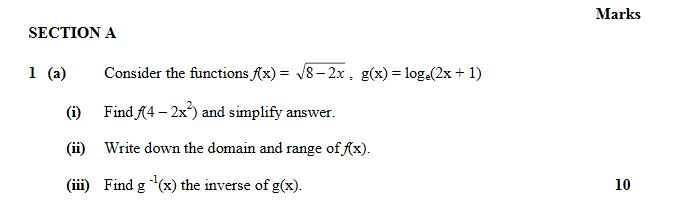
\includegraphics[width=0.9\linewidth]{Week7tut1}
\end{figure}

\subsection*{Question 25 : Functions - Part B}
\begin{figure}[h!]
	\centering
	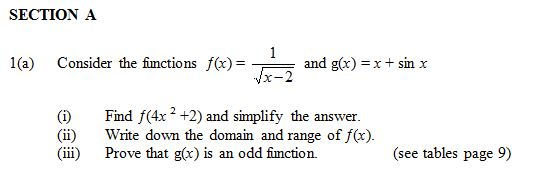
\includegraphics[width=1\linewidth]{Week7tut2}
\end{figure}
%=========================== %
\newpage
\subsection*{Question 26 : Domain and Ranges of Functions}
% - https://en.wikibooks.org/wiki/Algebra/Functions#Domain_and_Range
% - http://www.regentsprep.org/regents/math/algtrig/ATP7/fogprac.htm
Find the domain and the range of the functions:
\begin{multicols}{2}
	\begin{enumerate}[(i)]
		%number 1
		\item $f( x )= x - 2$ \,\, $g( x )= -2 x$
		
		%number 2
		\item $f( x )= x^2 - 4$\,\, $g( x )= - x^2 - 4$
		
		%\item $f( x )= x^2 - 2$, $g( x)= -0.5 x^2 - 2 x$
		
		%\item $f( x )= x^3$ , $g( x )= - x^3 - 4 x^2 - 4 x$
		
		\item $f( x )= \sqrt{x}$ \,\, $g( x )= \sqrt{x - 2}$
		
		%\item $f( x )= \sqrt{x +2}$ , $g( x )=  \sqrt{x - 2}-1$
		
		
		%number 4
		\item $f( x ) =  \sin x$ \,\, $g( x ) =  -2 \sin x$
		
		%number 5
		\item $f( x ) =  \cos x$ \,\, $g( x ) =  \cos^2(x)$
		
		%number 6
		\item $f( x ) =  e^{x}$\,\, $g( x) =  e^{x}- 2$
		
		
		%\item $f( x ) =  e^{-x}$, $g( x) =  e^{-x}- 2$
		%
		%
		%\item $f( x ) =  2 e^x$, $g( x ) = \frac{1}{e^x - 1}$
		%
		%
		%\item $f( x ) = | x |$, $g( x) =  | x - 2|$
		%
		%\item $f( x ) = | x |- 2$, $g( x) =  | x - 3 |- 1$
		
	\end{enumerate}
\end{multicols}		\smallskip
\subsection*{Question 27 : Domain and Ranges of Functions}
Find the domain and the range of the functions:
\begin{multicols}{2}
	\begin{enumerate}[(i)]
		\item $f(x) = 8 - 2 \sin(x)$ 	
		
		\item $f(x) = 5 - 2 \cos(2x)$ 
		\item $f(x) =  2 \cos(x)- 6$ 
		
		\item $f(x) = 7 + 2 \sin(3x)$ 
		
		\item $f(x) = |5\sin(x)|$ 
		
		\item $f(x) = \cos^2(x) +  \sin^2(x)$ 
		\item $f(x) = \cos^2(x) -  \sin^2(x)$ 
	\end{enumerate}	
\end{multicols}		
\smallskip
\subsection*{Question 28 : Evaluation of trigonometric values}
Evaluate the following values. \textit{you may use your calculator.}
\begin{multicols}{2}
	\begin{itemize}
		\item[(i)] $\cos (\pi/2)$
		\item[(ii)] $\sin (3\pi/4)$
		
		\item[(i)] $\tan (\pi/6)$
		\item[(ii)] $\cos (1.5 \pi)$
	\end{itemize} 
\end{multicols}
\bigskip	


\newpage
\subsection*{Question 29 : Composite Functions}
Determine the values of $f \circ g(2)$ and $g \circ f(x)$. Henxe or otherwise, evaluate $f \circ g(2)$ and $g \circ f(2)$.
\begin{multicols}{2}
	\begin{enumerate}[(i)]
		\item $f(x) = X^2 + 1$ and $g(x)= 2x$
		\item $f(x) = \sqrt{x+1}$ and $g(x)=x^2$
		\item $f(x) = x^2-1$ and $g(x) = 2x+1$
		
		\item $f(x) = 5x $ and $g(x)=x^2+1$
		\item $f(x) = -4x+9$ and $g(x) = 2x-7$
		%	\item $f(x) = -4x+9$ and $g(x) = 2x-7$
		\item $f(x) = e^x$ and $g(x)=\ln(x)$
		\item  $f(x) = x^2+1$ and $g(x) = 1-3x$
		\item $f(x) = \sin(\pi x)$ and $g(x) = 2x+1$
	\end{enumerate}	
\end{multicols}	
\medskip

\subsection*{Question 30 : Inverse Functions}

\begin{multicols}{2}
	\begin{enumerate}[(i)]
		\item	$f(x) = 2x$
		\item	$f(x) =e^x$
		\item	$f(x) = x-3$
		
		\item	$f(x) =\cos(x)$
		\item	$f(x) = \sin^{-1}(x)$
		\item  ${f(x) = \displaystyle \frac{1}{x-1}}$
		
		\item	$f(x) = x^2+2$
		\item	$f(x) = \sin^{-1}(2x)$
		\item	$f(x) = 3 e^{2x}$
		\item $f(x) = \sqrt{2x+3}$
		\item $f(x) = \log_e{4x}$
		\item $ \displaystyle f(x) = \frac{-2}{x-5}$
	\end{enumerate}	
	\smallskip
\end{multicols}
\noindent \textbf{Selected Solution}
\begin{enumerate}[(i)]
	\item For the function $f(x) = 2x$ the inverse function is $f^{-1}(x) = x/2$.
	\item For the function	$f(x) =e^x$ the inverse function is  $f^{-1}(x) = \log_e(x) = \ln(x)$.
	\item For the function	$f(x) = x-3$ the inverse function is $f^{-1}(x) = x+3$
	
	\item For the function	$f(x) =\cos(x)$ the inverse function is $f^{-1}(x) = \cos^{-1}(x)$.
	\item For the function	$f(x) = \sin^{-1}(x)$ the inverse function is $f^{-1}(x) = \sin(x)$.
	
	
\end{enumerate}
\newpage
%===========================================================================================%


\subsection*{Question 32 : Introduction to Integration}

\begin{figure}[h!]
	\centering
	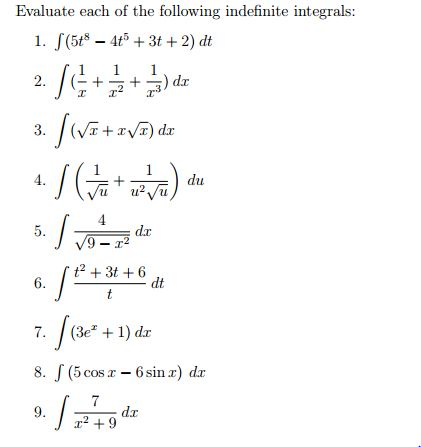
\includegraphics[width=0.9\linewidth]{Question19integration1}
\end{figure}

%=================================================================================== %


%==============================================================================%



<<<<<<< HEAD
=======
%============================================================= %
\newpage
\section*{MA4702 Integration}


\begin{figure}[h!]
	\centering
	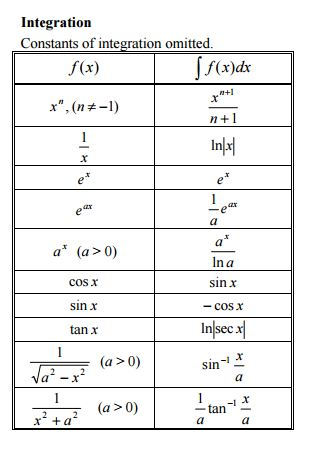
\includegraphics[width=0.55\linewidth]{integrationtabless}
\end{figure}



%Example
%
%\[\int_1^3 9 dx = 9(3-1)=9\cdot 2 = 18.\]
%\[\int_{-2}^6 11 dx = 11(6-(-2))=11\cdot 8 = 88.\]
%\[\int_{2}^{17} 0 dx = 0\cdot(17-2) =0.\]


Addition and Subtraction Rules of Integration
\[\int_a^b (f(x) + g(x)) dx = \int_a^b f(x) dx + \int_a^b g(x) dx.\]

\[\int_a^b (f(x) - g(x)) dx = \int_a^b f(x) dx - \int_a^b g(x) dx.\]


%Example
%
%From above $\int_1^3 9 dx =  18$ and $\int_1^3 2x^2 dx = \frac{52}{3} $so
%
%\[\int_1^3 (2x^2 + 9)dx = \int_1^3 2x^2 dx + \int_1^3 9 dx = \frac{52}{3} + 18 = \frac{106}{3},\]
%\[\int_1^3 (2x^2 - 9)dx = \int_1^3 2x^2 dx - \int_1^3 9 dx = \frac{52}{3} - 18 = -\frac{2}{3}.\]
%
%Example
%
%\[\int_0^2 4x^2 + 14 dx = 4\int_0^2 x^2 dx + \int_0^2 14 dx = 4 \cdot \frac{1}{3}(2^3-0^3) + 2 \cdot 14 = \frac{32}{3} + 28 = \frac{116}{3}.\]

\subsection*{The Power Rule for Integration}
The power rule for derivatives can be reversed to give us a way to handle integrals of powers of x. Since

\[\frac{d}{dx} x^n = n x^{n-1},\]

we can conclude that

\[\int n x^{n-1} \, dx = x^n + C,\]

or, a little more usefully,

\[\int x^n \, dx = \frac{x^{n+1}}{n+1} + C\]
\subsection*{Question 33 : Introduction to Integration}
%=========================== %

\subsubsection*{Part A}
Using appropriate substitutions, evaluate the indefinite integrals:

\begin{multicols}{2}
	\begin{enumerate}[(i)]
		
		\item 
		\[ \int (s - 4)^5 ds \]
		\item 
		\[ \int 
		\frac{3}{(x + 1)^4 }dx\]
		\item 
		\[\int 
		(2y + 3)(y^2 + 3y + 2)^2 dy\]
		
	\end{enumerate}
\end{multicols}

\subsubsection*{Part B}
Using appropriate substitutions, evaluate the indefinite integrals:
\begin{multicols}{2}
	\begin{itemize}
		
		\item[(i)]	
		\[\int 3x^2 (x^3+1)^5 \, dx\]
		
		\item[(ii)]
		\[\int x^4 \sin(x^5) \, dx\]
	\end{itemize}
\end{multicols}
\bigskip
%============================================================================================= %



%================================================= %
\subsection*{Question 43 : Definite Integrals}
Evaluate the following definite integrals 

\begin{enumerate}[(i)]
	
	\item 
	% - Lecture Notes Definite Integral
	% Examples 5 to 7
	Find the area between $f(x) = x^2 + 4x $ and the $x-$axis between 
	$x=-4$   and $ x=3$.
	
	\item Calculate the following:
	\[ \int^{1}_{0} \frac{4x^3}{x^4+1} dx \]
	
	
	\item Evaluate 
	
	\[ \int^{\frac{\pi}{2}}_{0} \cos^4(x) \sin(x) dx \]
\end{enumerate}

>>>>>>> 7dab53591cb406d2b3340a7bd90cbbebeb4d53b7

\subsection*{Question 44 : Integration : Partial Fraction Expansion Questions}
\begin{itemize}
	\item Suppose we have to integrate the following expression.
	\[\int \frac {1}{x+1} +\frac{1}{x-2} dx \]
	\item The integral of both individual terms are $ ln (x+1) $ and $ln (x-2) $
	
	\item The overall answer is therefore 
	
	\[ \int \left( \frac{1}{x+1} +\frac{1}{x-2}\right)\; dx \; =\; \ln (x+1) + \ln (x-2) + c\]
	
	\item Further simplifcations are possible, but you will get full marks once you get to there.
	\item As we covered this extensively at the start of the semester, You should expect a question like this.
\end{itemize}

%============================================================================%
% - http://math.gmu.edu/~memelian/teaching/Fall08/partDerivExamples.pdf

\subsection*{Question 45 : Applications of Integration - Electrical Circuits}
\begin{figure}[h!]
	\centering
	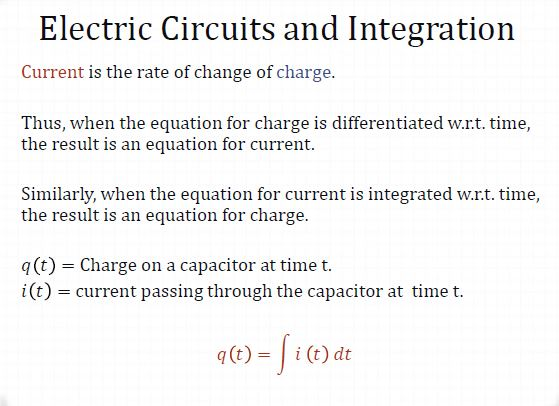
\includegraphics[width=0.6\linewidth]{circuits}
	
\end{figure}

\begin{enumerate}
	\item A current $i(t) = 4e^{-2t}$
	passes through a capacitor at
	time $t$. The capacitor is
	uncharged initially. Find the
	charge $q(t)$ at all times t.
	%-----------------------------------------------------%
	\item 
	A current $i(t) = 5 + 6 \sin 3t$
	passes through a capacitor at
	time $t$.
	The capacitor is uncharged at
	time $t=0$. Find the charge
	$q(t)$ at all times $t$. \textbf{\textit{2001 Q.3(b)}}
\end{enumerate}

%================================================================================%
\subsection*{Question 46 : Combined Integration Question (Exam Standard)}
% %\textit{This is an exam standard question. We will look at this in Week 13 (i.e. Revision Week)}

\begin{itemize}
	\item[(i)] 
	Evaluate the following indefinite integral: 
	\[\int 3x^2 +2e^x -1 dx\] 
	\item[(ii)] Evaluate the following definite integral: 
	\[\int^{9}_{4} \frac{1}{\sqrt{x}} dx\] 
	\item[(iii)] Find \[\int \bigg(e^{4x} + \cos(3) + \frac{1}{x^2} \bigg)dx\]
	
	\item[(iv)] The area enclosed between the curve $y=cos(x)$ and the x-axis between $x=0$ and $x= \frac{\pi}{3}$
\end{itemize}



\subsection*{Question 47 : Definite Integrals (Worked Example) }
\begin{framed}
	
	\noindent Consider the integral
	
	
	\[\int_{0}^2 x \cos(x^2+1) \,dx\]
	By using the substitution $u = x^2 + 1$, we obtain $du = 2x dx$ and
	
	\[	\int_{0}^2 x \cos(x^2+1) \,dx \qquad	= \frac{1}{2} \int_{0}^2 \cos(x^2+1) 2x \,dx \]
	\[	= \frac{1}{2} \int_{1}^{5}\cos(u)\,du  \qquad	= \frac{1}{2}\bigg(\sin(5)-\sin(1)\bigg).\]
\end{framed}
\bigskip

\newpage

\subsection*{Question 48 : Area Between Curves and Lines}
%=======================================================================%
\begin{enumerate}[(i)]
	\item (2005) Find the area bounded by the curves $y = x^2$ and $y = 2 – x^2$. 
	
	\item (2006) Find the area bounded by the curve $y = x^2 – 6x + 5$ and the line $y = x – 5$.
	
	\item (2007) Find the area bounded by the curves defined by $y = x^2 – 4$ and $y = 4 – x^2$. 
	
	\item (2008) Find the area bounded by the curve $y = x^2- 1$ and the line $y = 4x – 1$.
	
	\item (2009 ) Find the area bounded by the curve $y = 5x –x^2$ and the line $y = 2x$.
	
	\item (2010) Find the area enclosed by the curve $y = 4 –x^2$ and the line $y = x +2$.
\end{enumerate}
\bigskip
%============================================================================================= %

\subsection*{Question 49 : Integration : Partial Fraction Expansion Questions}
\begin{itemize}
	\item Suppose we have to integrate the following expression.
	\[\int \frac {1}{x+1} +\frac{1}{x-2} dx \]
	\item The integral of both individual terms are $ ln (x+1) $ and $ln (x-2) $
	
	\item The overall answer is therefore 
	
	\[ \int \left( \frac{1}{x+1} +\frac{1}{x-2}\right)\; dx \; =\; \ln (x+1) + \ln (x-2) + c\]
	
	\item Further simplifcations are possible, but you will get full marks once you get to there.
	\item As we covered this extensively at the start of the semester, You should expect a question like this.
\end{itemize}

%============================================================================%
% - http://math.gmu.edu/~memelian/teaching/Fall08/partDerivExamples.pdf

\newpage

\subsection*{Question 50a : Partial Derivatives}
\begin{itemize}
	\item[(i)] Find ${ \partial{z} \over \partial{x} }, { \partial{z} \over \partial{y} }, { \partial^2{z} \over \partial{x}\partial{y} }$ 
	of the function $z = 2x^2y+4xy^3+5x^2$.		             
	
\item (Rest of Question removed)
%	10
\end{itemize}
%============================================================================%


\subsection*{Question 50b : Partial Derivatives}


Solve for $\displaystyle{\partial f/\partial x}$ and $\displaystyle{\partial f/\partial y}$ if \[f(x,y)= ln(xy) +sin(x) = ln(x) + ln(y)+ sin(x)\].

%\noindent \textbf{Solution :}
%\[\partial f/\partial x = \]
%\[\partial f/\partial y = \]



\subsection*{Exercise 51 : (Worked Example)} 
Solve for $\displaystyle{\partial  f/\partial x}$ and $\displaystyle{\partial f/\partial y}$ if \[f(x,y) = -x^2+y\]

\noindent \textbf{Solution :}
\[ \partial f/\partial x = -2x \]
\[ \partial f/\partial y = 1\]


\subsection*{Question 52 : Partial Derivatives}
Determine all first order and second order partial derivatives of each of the following.
\begin{multicols}{2}
	\begin{enumerate}[(i)]
		
		\item $\displaystyle{f(x, y) = 3x + 4y}$
		
		\item $\displaystyle{f(x, y) = xy^3 + x^2y^2}$
		\item $\displaystyle{f(x, y) = x^3y + e^x}$
		
%		\item $\displaystyle{f(x, y) = xe^{2x+3y}}$
%		
%		%	\item $\displaystyle{f(x, y) = \frac{x - y}{x+y}} $
%		
%		\item $\displaystyle{f(x, y) = 2x \sin(x^2y)}$.
%		
%		
	\end{enumerate}
\end{multicols}


%================================================================================ %

\newpage

%\chapter{Curvesketching}
\subsection*{Question 53 : Curve Sketching}
\begin{itemize}
	\item[Ex. 1]
	\begin{itemize}
		\item[(i)] Find the $y$ intercept of the function $y=f(x)$.
		\item[(ii)] Show that $(\sqrt{3},1)$ is a stationary point of the function. Find the other two stationary points and classify all
		three points as local maxima or minima.
		\item[(iii)] Find the two inflection pints of $f(x)$.
		\item[(iv)] Find the $x$ values for which is $y=f(x)$ is concave up/down.
		\item[(v)] Determine the behaviour of $y$ as $x \rightarrow + \infty$ and as $x \rightarrow -\infty$ 
		\item[(vi)] Sketch the graph of $y = f(x)$ indicating clearly the features of the curve obtained in aprts (i) to (v) of this quesiton.
	\end{itemize}
	
	
	\item[Ex. 2] Find $\alpha$ and $\beta$ so that the function 
	
	\begin{displaymath}f(x) = \alpha x^3 + \beta x^2+1\end{displaymath}
	
	has a point of inflection at  $\displaystyle \left(-1,2\right)$
\end{itemize}



\subsection*{Question 54 : Curve Sketching}
\subsubsection*{Past Paper Question -  Summer 04/05}
\begin{figure}[h!]
	\centering
	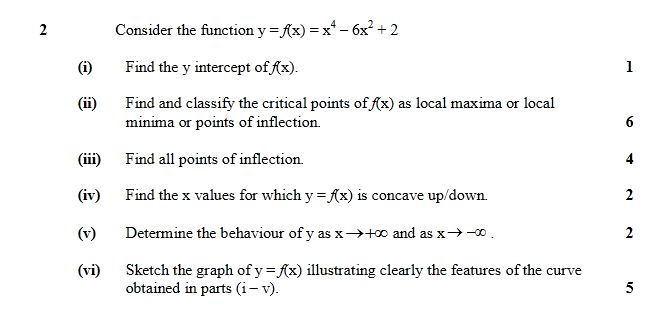
\includegraphics[width=0.87\linewidth]{curvesketching0405}
	
\end{figure}

\subsection*{Question 56 : Curve Sketching}
\subsubsection*{ Past Paper Question - Summer 05/06}
\begin{figure}[h!]
	\centering
	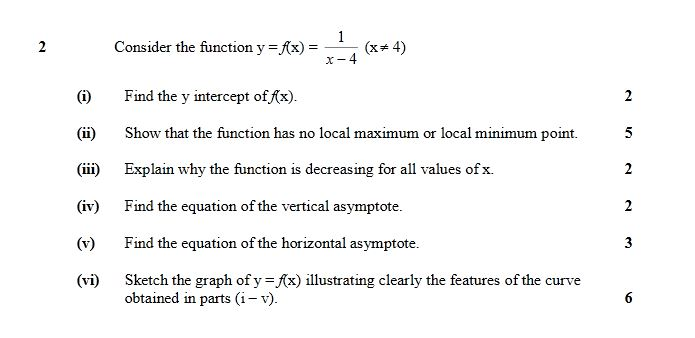
\includegraphics[width=0.87\linewidth]{curvesketching0506}
	
\end{figure}
\newpage
\subsection*{Question 56 : Curve Sketching}

This is Curve Sketching Example 3 from the lectures. The entirety of the material covered by this question is examinable in the End-Of-Semester exam.

\begin{figure}[h!]
	\centering
	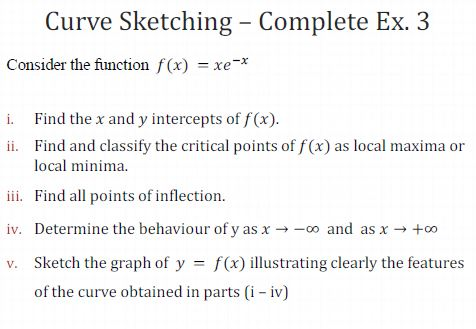
\includegraphics[width=0.6\linewidth]{Q17curvesketching}
	
\end{figure}
\subsection*{Question 57 : Curve Sketching}

This is Curve Sketching Example 4 from the lectures. The entirety of the material covered by this question is examinable in the End-Of-Semester exam.
\begin{figure}[h!]
	\centering
	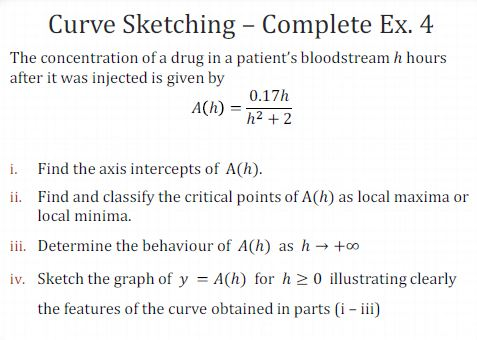
\includegraphics[width=0.6\linewidth]{Q18curvesketching}
	
\end{figure}

\newpage
\subsection*{Question 58 : Curve Sketching}
Consider the function $y = f(x) = x^4 – 6x^2 + 2$
\begin{itemize}
	\item[(i)] Find the y intercept of f(x). 
	
	\item[(ii)] Find and classify the critical points of f(x) as local maxima or local minima or points of inflection. 
	
	\item[(iii)] Find all points of inflection. 
	
	\item[(iv)] Find the x values for which y = f(x) is concave up/down. 
	
	\item[(v)] Determine the behaviour of y as $x \to +\infty$ and as $x \to -\infty$. 
	
	\item[(vi)] Sketch the graph of y = f(x) illustrating clearly the features of the curve obtained in parts (i – v). 
\end{itemize}




\end{document}
